\documentclass[11pt]{article}
\usepackage{amssymb,amsfonts,amsmath}
\usepackage{algorithmic}
\usepackage[pdfborderstyle={/S/U/W 1}, allbordercolors={0 0 0}]{hyperref}
\usepackage[pdftex]{graphicx}
\usepackage[super]{nth}

\pagestyle{plain} \textwidth 18.0cm \topmargin -3.0cm \textheight
27.0cm \oddsidemargin -1.0cm
\parindent 0.0cm
\font\myfont=msbm10 scaled \magstep1
\newcommand{\pbeg}{\hspace*{0.8cm}}
\newcommand{\magtodb}[1]{20\times\log\left(#1\right)}
\newcommand{\dbtomag}[1]{10^{(#1)/20}}
\newcommand{\underscore}{\underline{ }}
\newcommand{\bigspace}{\vspace{0.4cm}}
\newcommand{\smallspace}{\vspace{0.2cm}}

\begin{document}
\title{CV}
\date{}
\author{Bilal ACAR}
\let\thefootnote\relax

\pagestyle{empty}
\begin{tabular}{l c c c c c c c c c c c p{3cm}}
\begin{tabular}{p{8cm} l}
\vspace{40pt}
\Huge Bilal ACAR \normalsize & \\
\vspace{8pt}
bilal.acar.a@gmail.com & \\
\textbf{+31 65 469 85 63} & \\
Lenghengang 15A, Dordrecht, Zuid Holland, The Netherlands, 3311NP &
\end{tabular}
& & & & & & & & & & & &
\raggedleft
\vspace{-40pt}
%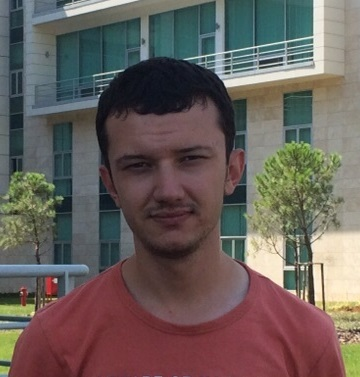
\includegraphics[width=4cm,keepaspectratio]{figs/res.jpg}
\vspace{-40pt}
\end{tabular}

\bigspace
\begin{tabular}{p{18cm}}
\textbf{Work Experience} \\
\hline
\end{tabular}


\begin{tabular}{p{5.5cm} p{12.5cm}}
\\
2020 March - Present:   & Amazon Web Services \textit{Vancouver-Canada}: Software Development Engineer \\
							 &
\begin{itemize}
\setlength\itemsep{0em}
\vspace{-15pt}
\item Working in Amazon MQ for RabbitMQ team
\item Been a part of the development team that launched Amazon MQ for RabbitMQ
\item Designed and implemented several key components of RabbitMQ service, such as restart workflow, maintenance windows, ops tools, etc.
\item Currently leading Operations Excellence track. Triaging and prioritizing operations improvement tickets.
\vspace{-10pt}
\end{itemize}\\
2019 April - 2019 October:   & Ingenico ePayments \textit{Hoofddorp-The Netherlands}: Software Developer \\
							 &
\begin{itemize}
\setlength\itemsep{0em}
\vspace{-15pt}
\item Worked in travel team which is responsible for travel industry (airlines, travel agencies, booking sites, etc) e-payments
\item Re-implemented legacy BSP (Billing and Settlement Plan) application using modern technologies such as Java 11, Kotlin, and Spring Boot
\item Worked in a vertical team which is responsible for writing the code, maintaining CI/CD pipelines, deploying software to production, and technical support
\vspace{-10pt}
\end{itemize}\\
2016 May - 2019 March:       & Connectis R\&D B.V. \textit{Rotterdam-The Netherlands}: Software Developer \\
							 &
\begin{itemize}
\setlength\itemsep{0em}
\vspace{-15pt}
\item Developed and maintained Java/Kotlin codebase of Connectis Identity Broker and its various components
\item Worked on several products of the company, such as OAuth server, identity broker to identity provider connection, configuration, attribute provider, etc.
\item Worked on the implementation of attribute provider which is an implementation of SCIM (\url{http://www.simplecloud.info/}) protocol. The whole implementation is done using Kotlin as programming language and MongoDB as database
\vspace{-10pt}
\end{itemize}\\
2014 July - 2016 April:      & SAP Innovation Center Turkey \textit{\.{I}stanbul-Turkey}: Software Developer \\
							 &
\begin{itemize}
\setlength\itemsep{0em}
\vspace{-15pt}
\item Developed regression and association algorithms (support vector regression and apriori algorithms) as a member of Turkish Airlines Predictive Maintenance Team
\item Developed predictive analytics component (implemented power prediction and event prediction algorithms) of SAP IT Operations Analytics (ITOA) product as a member of the same team
\item Done handover of predictive analytics component of ITOA and attended workshops in Walldorf, Germany to finalize the handover
\vspace{-10pt}
\end{itemize}\\
\end{tabular}
\begin{tabular}{p{5.5cm} p{12.5cm}}
2013 July - 2014 June:       & Bo\u{g}azi\c{c}i University \textit{\.{I}stanbul-Turkey}: Research Assistant \\
							 &
\begin{itemize}
\setlength\itemsep{0em}
\vspace{-15pt}
\item Developed multi-core simulators for nano-network simulations using Java
\item Used the simulator to optimize data rate of molecular communication networks
\item Received research project scholarship from Bo\u{g}azi\c{c}i University Scientific Research Projects (2013).
\vspace{-10pt}
\end{itemize}\\
\end{tabular}

%\bigspace

\begin{tabular}{p{18cm}}
\textbf{Education} \\
\hline
\end{tabular}


\begin{tabular}{p{5.5cm} p{12.5cm}}
\\
2007 September - 2013 January:
&	Bo\u{g}azi\c{c}i University - Computer \& Industrial Engineering (Double Major)\\
&	\textbf{GPA: 3.68/4.00 (\nth{3} Highest GPA in Computer Engineering \& \nth{4} Highest GPA in Industrial Engineering)}\\


2003 September - 2007 June:
&	D\"{u}zce Science High School\\
&	\textbf{GPA: 96.51/100 (\nth{3} Highest GPA)}
\end{tabular}

%\pagebreak

\begin{tabular}{p{18cm}}
\textbf{Skills} \\
\hline
\end{tabular}

\bigspace
\begin{tabular}{p{18cm}}
\textit{\textbf{Programming Languages:}}
\vspace{-7pt}
\begin{itemize}
\setlength\itemsep{0em}
\item Proficient: Java, Kotlin, SQL
\item Familiar: C/C++, R, Matlab, JavaScript, C\#
\end{itemize}
\end{tabular}

\begin{tabular}{p{18cm}}
\textit{\textbf{Development Tools, Platforms, and SCM:}} \\
Intellij, Git, Mercurial, Maven, Guice, Spring Boot, Ansible
\end{tabular}

\bigspace

\begin{tabular}{p{18cm}}
\textit{\textbf{Methodologies:}} \\
Agile, Scrum, LeSS, Spotify Model
\end{tabular}

\bigspace

\begin{tabular}{p{18cm}}
\textit{\textbf{Databases and Enrivonments:}} \\
MongoDB, PostgreSQL, Linux (Ubuntu)
\end{tabular}

\bigspace

\begin{tabular}{p{18cm}}
\textit{\textbf{Languages:}}\\
Turkish (Native), English (Fluent)
\end{tabular}

\bigspace

\begin{tabular}{p{18cm}}
\textit{\textbf{Background in Machine Learning:}}\\
Clustering algorithms (Agglomerate hierarchical clustering, K-Means), Classification algorithms (Support vector machine, Decision tree algorithms), Regression algorithms (Polynomial regression, Support vector regression), Association algorithms (Apriori algorithm), Preprocessing algorithms (Principal component analysis)
\end{tabular}


\begin{tabular}{p{18cm}}
\textit{\textbf{Background in Operations Research:}}\\
Linear optimization, non-linear optimization, stochastic optimization, heuristic algorithms (Simulated Annealing, Tabu Search, Genetic Algorithm, swarm optimization)
\end{tabular}

\bigspace
\begin{tabular}{p{18cm}}
\textbf{Selected Projects and Publications} \\
\hline
\end{tabular}

\begin{itemize}
\item \textit{Mongeez - Change set management for MongoDB}: Worked on a fork of mongeez project on github which handles change set management for MongoDB. The project was only using Java drivers eval method for database operations, which requires a special user in the database. I added mongo shell support for database operations and command line interface on top of the library for easy out of box use. Github page of the project: \url{https://github.com/bzacar/mongeez}
\item \textit{CMPE/IE 492 Project in Computer \& Industrial Engineering (BS Graduation Project)}: An Optimization Approach for Zone-Based Sensing Scheduling in Cognitive Radio Networks. Developed a simulation and optimization tool in Java. The application provides a Swing GUI and a console interface. Github page of the project: \url{https://github.com/bzacar/cmpe492-cr-sensing-simulation}
\item Bilal Acar, M. Akif Ersoy, H. Birkan Yilmaz, Salim Eryigit, Tuna Tugcu. \href{http://www.computer.org/csdl/proceedings/iscc/2012/2712/00/IS273.pdf}{Zone-based Spectrum Sensing In Cognitive Radio}. In \textit{IEEE Symposium on Computers and Communications (ISCC)}, 2012.
\end{itemize}

\begin{tabular}{p{18cm}}
\textbf{References} \\
\hline
\vspace{0.2cm}
References available upon request.
\end{tabular}


\end{document}
